%%%%%%%%%%%%%%%%%%%%%%%%%%%%%%%%%%%%
% KTHEEtitlepage_ex.tex
%
% Example of how to use the KTHEEtitlepage package.
% 
% Mats Bengtsson,  7/8 2006
%%%%%%%%%%%%%%%%%%%%%%%%%%%%%%%%%%%%
\documentclass[a4paper]{article}

\usepackage[utf8]{inputenc}
\usepackage[ireport]{KTHEEtitlepage}
\usepackage{graphicx}

% Packages used in the main document for this particular example:
\usepackage{url}

\begin{document}

\begin{abstract}
This paper tests different readability algorithms in different languages. Readability is simply how easy a text can be read and understood. The tests conducted was done on texts in both Swedish and English within the same subject where readability is expected to be the same. Three algorithms was tested, Coleman-Liau index, Läsbarhetsindex and Automated Readability Index. 
\end{abstract}
\newpage

\tableofcontents
\newpage

% Everything below is exactly as for a normal document and 
% the layout of that document should not be affected in any
% way by the title page.

% -----------------------------------INTRODUCTION-----------------------------------
\section{Introduction}

Readability is the ease in which text can be read and understood. Various factors to define readability have been used, such as:

\begin{itemize}
  \item Speed of perception
  \item Perceptibility at a distance
  \item Perceptibility in peripheral vision
  \item Visibility
  \item The reflex blink technique
  \item Rate of work (e.g., speed of reading)
  \item Eye movements
  \item Fatigue in reading, etc \ldots
\end{itemize}

Thus there are many ways to look upon readability and various ways in measuring it. The Oxford dictionary defines the word "readable", from which the word "readability" derives, as:

\begin{quote}
    \begin{enumerate}
        \item Able to be read deciphered; legible: a code which is readable by a computer readable copies of very old newspapers
        \begin{enumerate}
            \item Easy or enjoyable to read: a marvellously readable book
        \end{enumerate}
    \end{enumerate}
\end{quote}

For our purposes readability will be defined as the ease in which a text can be read and understood. This definition is coming from "Legibility of Print" \cite{tinker63} and is chosen due to its simplicity and its focus on understanding. 

How to determine readability varies and this introduces a problem which have to be taken into major consideration in this paper. We will study existing algorithms, which all use the their own definition of readability and their own methods on how to measure it. The most common factors in these existing algorithms are: 

\begin{itemize}
    \item The total amount of words
    \item The length of sentences
    \item The amount of words defined as complicated
    \item The amount syllables, etc \ldots
\end{itemize}

\subsection{Statement of the problem}
Despite  using  the  right  factors  one  must  also determine how the chosen factors relate to each other to give the text its readability. The question examined in this report is how readability algorithms perform when processing texts written in different, not too distantly related, human languages. The languages swedish and english was chosen for the research due to their resemblance. 

To do this texts with the same readability in both swedish and english have to be evaluated with the same algorithms. As algorithms use different variables to determine readability this might pose a problem with different languages.

The problem is as follows:
\newline
\newline
\textbf{How do readability algorithms perform when processing texts written in multiple languages?}
% -------------------------------BACKGROUND-----------------------------------
\section{Readability evaluation algorithms}

In this section some readability algorithms shall be introduced. These algorithms were chosen due to the width of their use and their fit for ours. The parameters most important for our purpose was simplicity, usage and language. Simplicity since it is essential when the purpose is to use the algorithm on a various of languages. The simplicity main focus we have are the ease in which to acquire the variables needed to compute the formula.

\subsection{Läsbarhetsindex (LIX)}

LIX was developed by Carl-Hugo Björnson\cite{reck}. It was made for the Swedish language but is said to work with most Western European languages\cite{brown}. The score is calculated by a formula using the number of words, periods and long words. A long word is for this instance defined as a word with more than six characters. The formula is as follows\cite{reck, bjornsson68}:

\begin{equation}
    LIX = W/S+(L*100)/W
\end{equation}
\emph{W:= The total amount of words}\\
\emph{S := The total amount of sentences}\\
\emph{L := The total amount of long words}\\

Hence the formula can be defined as the average amount of words per sentence added with the percentage of long words by the total amount of words. The result of the LIX formula can be translated by the following table:

\begin{equation}
    \begin{tabular}{c|c}
        \textless 25    &   Childrens books, etc\\
        25-30   &   Simple texts \\
        30-40   &   Normal texts / Fiction \\
        40-50   &   Factual texts\\
        50-60   &   Technical texts \\
        \textgreater 60    &   Difficult technical texts / Research / Dissertations
    \end{tabular}
\end{equation}

\subsection{Flesch-Kincaid}

The Flesch readability scale was developed by Rudolf Flesch in 1948 and is based on school text of different grades\cite{navy75}. This algorithm has an inverted scale compared to other algorithms, high points means it is easy to read and low the opposite. This test is used in some of the United States agencies, for example the department of defense used it to assess the difficulty in technical manuals before it was adopted as standard assessment of readability\cite{navy75, mcclure87}.

The Flesch Reading Ease formula calculates readability as follows:

\begin{equation}
F = 206.835 - 1.015(W/S) - 84.6(Y/W)
\end{equation}
\emph{W := Total amount of words}\\
\emph{S := Total amount of sentences}\\
\emph{Y := Total amount of syllables}\\

The Flesch-Kincaid readability formula is an improved version of the Flesch Reading Ease formula. The formula was created by Flesch and John P. Kincaid and unlike the Flesch Reading Ease formula the Flesch-Kincaid formula returns a value corresponding to a grade level\cite{navy75}. For example a score of 7.4 would indicate that the text in mention would have the readability understandable by an average student in the 7th grade in the United States or a student in year 7 in the United Kingdom. 

The Flesch-Kincaid formula calculates readability as follows:

\begin{equation}
FK = 0.39(W/S) + 11.8(Y/W) - 15.59
\end{equation}
\emph{W := Total amount of words}\\
\emph{S := Total amount of sentences}\\
\emph{Y := Total amount of syllables}\\

\subsection{Coleman-Liau}

The Coleman-Liau formula was developed by Meri Coleman and T. L. Liau and was published in 1975. The Coleman-Liau formula differs from the Flesch-Kincaid formula in such way as it does not rely on syllables\cite{coleman75}. Using syllables is said to be more accurate but accuracy can be outweighed by simplicity. This perticulat formula was intended for use with computers which gives weight to simplicity in parsing over accuracy\cite{coleman75}. A result from the Coleman-Liau formula corresponds just like the Flesch-Kincaid formula, to a United States grade level\cite{coleman75}. 

The Coleman-Liau index calculates readability as follows:

\begin{equation}
CLI = 0.0588L - 0.296S - 15.8
\end{equation}
\emph{L := Average amount of letters, numbers and punctuation marks per 100 words}\\
\emph{S := Average amount of sentences per 100 words}\\
\newline
, hence:

\begin{equation}
CLI = 5.88(L/W) - 29.6(S/W) - 15.8
\end{equation}
\emph{L := Total amount of letters, numbers and punctuation marks}\\
\emph{W := Total amount of words}\\
\emph{S := Total amount of sentences}\\

\subsection{Automated Readability Index (ARI)}
Automated readability index was developed to monitor electrical typewriters in real time. Like the Coleman-Liau formula ARI does not use syllables to compute readability and the result corresponds to the same United States grade level\cite{senter67}. It was developed for the United States Air Force to have an easy way to determine the ease which manuals and text books could be read\cite{senter67}.

ARI calculates readability as follows:

\begin{equation}
ARI = 4.71(L/W) + 0.5(W/S) - 21.43
\end{equation}
\emph{L := Total amount of letters, numbers and punctuation marks}\\
\emph{W := Total amount of words}\\
\emph{S := Total amount of sentences}\\

\subsection{SMOG readability formula}

SMOG was developed by Harry McLaughlin and is used widely, particularly in health care\cite{ley96}. It is said to be more accurate and simpler then earlier formulas\cite{laughlin69}. SMOG was made for the English language.A result from the SMOG formula corresponds to a United States grade level.
 The SMOG formula calculates readability as follows:

\begin{equation}
    SMOG = 1.0430\sqrt[2]{X*30/S}+3.1291
\end{equation}
\emph{X := The total amount of polysyllables}\\
\emph{S := The total amount of sentences}\\

SMOG should be applied to at least 30 sentences of a text, preferably in the beginning, middle and end to give a credible score\cite{laughlin69}.

% -----------------------------------METHOD-----------------------------------
\section{Method}
Some readability formulas suite the issue more than others. First of all formulas using syllables was excluded due to a problem when parsing texts in different languages. This problem is by the fact that syllables are defined in such a way that there is no easy way to read them with a computer\cite{coleman75}. Thereby the Flesch-Kincaid formula as well as SMOG was exluded. 

Second formulas relevant to both english and swedish are desirable. Since readability are most often adapted to english, due to the size of the language and the nationality of the scientists developing the formulas, it is not a problem to find formulas relevant for english. However swedish being a much smaller language, LIX is the only readability formula with a definite reliability to the swedish language. The readability formulas implemented are:
\begin{itemize}
    \item Läsbarhetsindex (LIX)
    \item Coleman-Liau (CLI)
    \item Automated Readability Index (ARI)
\end{itemize}
LIX, CLI and ARI all only uses variables that can be calculated by looking on individual characters, words and sentences without having to do any special interpretations when handling multiple languages. Being independent from language restrictions thereby makes these formulas suitable. They are also wildly spread and used which makes them more relevant to test and interesting to test.

The texts we have chosen to examine are Wikipedia articles, the Bible and "On the Origin of Species" by Charles Darwin\cite{darwinEN, darwinSV, bibleEN, bibleSV}. Wikipedia has the advantage of being easy to access and having a large amount of texts written in many different languages on the same subject. To generate a somehow accurate result with readability formulas larger texts are necessary. Since about 60\% of Wikipedia articles does not consist of more than a few sentences, most of them are not suitable for this research\cite{anderson12}. Therefor articles exclusively about countries was used due to the guarantee of getting articles with a more proper content. However the english Wikipedia articles almost always contain more content than the swedish translation, which would affect the scores negatively.

The Bible and "On the Origin of Species" was chosen because of the difference of genre and thereby writing. Also both sources has a large content and are easy to get in find languages. The problem with these sources is that they are not written by the same author, which causes the otherwise assumable likewise readability indexes to differ.

To parse the texts Python3 was used. This programing language was chosen because of it's simplicity and since there are no performace requirements. A Python library called "Wikipedia" collect the Wikipedia articles and a library called "Translate" which inherit from "Google Translate" is used not to translate the texts, but to translate the the country names to swedish. To calculate the amount of characters, words and sentences in a text regex is used. The Python regex library "re" contributes with the functionality needed. With this methods was created to calculate the amount of characters, words and sentences of the texts. With the variables sorted out the formulas was run on each individual text giving the result in a JSON file.


% -----------------------------------RESULT-----------------------------------
\section{Result}
The results were all calculated by the Python readability program using the appropriate libraries, as described. The main program is in the "readability.py" file which uses the "nations.py" for the Wikipedia article parsing. The program as whole can be found in Appendix A, and the data calculated by it can be found in Appendix B. 

\subsection{Average scores of Wikipedia articles}
To get an understanding of the large amount of readability scores an average score is calculated as an interpretation. To calculate the average scores a function to the Python program was added named "calc\_average". This function first calculates every single score and sum these, then it divide the sum by the amount of articles used.

The average scores are as follows:

\begin{itemize}
    \item \textbf{English}
    \begin{itemize}
        \item Coleman-Liau Index (CLI): \textbf{13.562801576949234}
        \item Automated Readability Index (ARI): \textbf{14.03930181327097}
        \item Läsbarhetsindex (LIX): \textbf{53.74258224186213}
    \end{itemize}
    \item \textbf{Swedish}
    \begin{itemize}
        \item Coleman-Liau Index (CLI): \textbf{16.490071197789494}
        \item Automated Readability Index (ARI): \textbf{12.95953472172705}
        \item Läsbarhetsindex (LIX): \textbf{49.79444013958571}
    \end{itemize}
\end{itemize}

\subsection{Scores of "On the Origin of Species"}
The method calculating the scores of "On the Origin of Species" is named "calc\_darwin". By running the method the following data was collected:

\begin{itemize}
	\item \textbf{English version}
	\begin{itemize}
		\item Amount of characters: \textbf{723035}
		\item Amount of words: \textbf{150763}
		\item Amount of long words: \textbf{37362}
		\item Amount of sentences: \textbf{4328}
	\end{itemize}
	\item \textbf{Swedish version}
	\begin{itemize}
		\item Amount of characters: \textbf{861388}
		\item Amount of words: \textbf{164724}
		\item Amount of long words: \textbf{45374}
		\item Amount of sentences: \textbf{5074}
	\end{itemize}
\end{itemize}

Using functions 1, 6, 7 and the data above, the following scores was given:

\begin{itemize}
    \item \textbf{English}
    \begin{itemize}
        \item Coleman-Liau Index (CLI): \textbf{11.549794047611151}
        \item Automated Readability Index (ARI): \textbf{18.57556662482323}
        \item Läsbarhetsindex (LIX): \textbf{59.616277084672305}
    \end{itemize}
    \item \textbf{Swedish}
    \begin{itemize}
        \item Coleman-Liau Index (CLI): \textbf{14.036399310361578}
        \item Automated Readability Index (ARI): \textbf{19.432075097258753}
        \item Läsbarhetsindex (LIX): \textbf{60.00979794469356}
    \end{itemize}
\end{itemize}

\subsection{Scores of the Bible}
The method calculating the scores of the Bible is named "calc\_bible". By running the method the following data was collected:

\begin{itemize}
	\item \textbf{English version}
	\begin{itemize}
		\item Amount of characters: \textbf{3224231}
		\item Amount of words: \textbf{790051}
		\item Amount of long words: \textbf{95726}
		\item Amount of sentences: \textbf{29813}
	\end{itemize}
	\item \textbf{Swedish version}
	\begin{itemize}
		\item Amount of characters: \textbf{3370368}
		\item Amount of words: \textbf{765993}
		\item Amount of long words: \textbf{113058}
		\item Amount of sentences: \textbf{55123}
	\end{itemize}
\end{itemize}

Using functions 1, 6, 7 and the data above, the following scores was given:

\begin{itemize}
    \item \textbf{English}
    \begin{itemize}
        \item Coleman-Liau Index (CLI): \textbf{7.079552687105011}
        \item Automated Readability Index (ARI): \textbf{11.041814966006733 }
        \item Läsbarhetsindex (LIX): \textbf{38.6166510154625}
    \end{itemize}
    \item \textbf{Swedish}
    \begin{itemize}
        \item Coleman-Liau Index (CLI): \textbf{7.941891949404237}
        \item Automated Readability Index (ARI): \textbf{6.242027017148239}
        \item Läsbarhetsindex (LIX): \textbf{28.655733697165452}
    \end{itemize}
\end{itemize}

% -------------------------------DISCUSSION-----------------------------------
\section{Discussion}
Evaluating readability will always come with problems as it is very hard to find a scale which cover all the existing aspects of it. The scales used by the most known formulas are given by matching the score to a large amount of data. Doing this will give a good value for an average human being but since no person is average evaluating text after using humans will present difficulties because readability is subjective and usually only works on large amounts of data. Having problems collecting suitable data to evaluate will pose a problem to get a trustworthy result. 

A problem is apparent with the data that is used from Wikipedia. Wikipedia articles are written by random users whom follow only a few rules when writing and the free text in the articles can vary wildly. This might have influenced the result if the articles was written by different authors using different writing techniques and therefore giving a not trustworthy result of readability. Also the length of the articles plays a part as the ones written in english tend to be more thorough and having a larger content than the respective article written in any other language. This will result in a wider base of data for the english result sets, for better or worse. Actions has been taken in order to prevent this by using articles about nations to minimize the difference of content size. However this will not remove the fact that the articles are not the same and can not be looked upon as such. To work the problem one would have to evaluate all the texts used by hand, which would be very time and resource consuming and neither the time or the resources existed for it to be an option. Even if it would be done there would still be no guarantee that the texts would be the same. This is of course something that regards all used sources, but it would not be unjustified to assume that the Wikipedia articles are more exposed to this problem due to the fact that anyone could have written the articles from Wikipedia, unlike the Bible and "On the Origin of Species".

The data collected from the Wikipedia articles shows that the readability corresponds to the middle of the scales used in each separate algorithm, as expected due to the fact that Wikipedia articles are factual texts. The LIX algorithm showed a difference of less than one percent comparing the result of the english texts to the swedish ones. The score also represented the level expected from Wikipedia articles. Looking at "On the Origin of Species" shows that the LIX score also corresponds to the expected level of readability and that there is a small difference between the results of the languages. This indicates that LIX works on texts from the middle and higher readability scales for both english and swedish. The unexpected result turned when applying LIX to the Bible. Although both scores would indicate that the Bible is fairly easy to read, they were in fact put in different section of the LIX table. The swedish score would indicate that the bible is a simple text while the english score would indicate that the bible has the readability of a normal text or fiction.

The ARI formula differed almost eight percent comparing english to swedish which would correspond to a year in the american school but is still a neglectable difference on the Wikipedia comparison and gives a simular difference for "On the Origin of Species". The minor difference in score would indicate that ARI and LIX are in fact applyable to both english and swedish. ARI simular to LIX only gives unexpected results when comparing the Bible in the different languages, which would indicate that the Bible swedish translation of the Bible varies much from the english one.

The Coleman-Liau formula differed slightly over seventeen percent between the languages on the Wikipedia articles and this is a relative large difference. Coleman-Liau is also the only one of the three algorithms that gives a higher result for Swedish on all three sources and the only one not to give a differing result on the readability of the Bible.

A recurring problem was the differing of the Bible readability results. However the CLI indicated differantly than the other two formulas, showing a similar result for both the swedish and the english versions. This could be an effect of CLI being the only one of the three readability formulas taking in account the amount of sentences per hundred words and the fact that the Bible is using a relatively different sentance structure in comparison to the other sources. The result of the CLI could indicate that the sentence structure used in the Bible would is a better fit for the CLI than for the ARI or for the LIX.

\subsection{Conclusion}


\newpage
% ------------------------------BIBLIOGRAPHY-------------------------------
\begin{thebibliography}{99}

\bibitem{bjornsson68}
  Carl-Hugo Björnsson,
  \emph{Läsbarhet}.
  Liber, Stockholm,
  1968.
  
\bibitem{reck}
  Ronald P. Reck and Ruth A. Reck,
  \emph{Generating and Rendering Readability Scores for Project Gutenberg Texts}.
  
\bibitem{brown}
  Jonathan C. Brown and Maxine Eskenazi,
  \emph{Student, Text and Curriculum Modeling For Reader-Specific Document Retrieval}.
  Carnegie Mellon University,
  Pittsburgh, PA.

\bibitem{falkenjack}
  Johan Falkenjack and Katarina Heimann Muhlenbock,
  \emph{Using the probability of readability to order Swedish texts}.
  2012.
  
\bibitem{tinker63}
  Tinker and Miles A,
  \emph{Legibility of Print}.
  Iowa State University Press, Iowa,
  1963.
  
\bibitem{navy75}
  Kincaid, J P ; Fishburne, Jr , Robert P ; Rogers, Richard L ; Chissom, Brad S,
  \emph{Derivation of New Readability Formulas (Automated Readability Index, Fog Count and Flesch Reading Ease Formula) for Navy Enlisted Personnel}.
  Naval Technical Training Command Millington TN Research Branch,
  1975.

\bibitem{mcclure87}
  McClure G,
  \emph{Readability formulas: Useful or useless. (an interview with J. Peter Kincaid.)}.
  IEEE Transactions on Professional Communications,
  1987.

\bibitem{coleman75}
  Coleman, M.; and Liau, T. L.,
  \emph{A computer readability formula designed for machine scoring}.
  Journal of Applied Psychology,
  vol. 60,
  1975.
  
\bibitem{senter67}
  E. A. Smith and R. J. Senter,
  \emph{Automated Readability Index}.
  Aerospace Medical Research Laboratories
Aerospace Medical Division
Air Force Systems Command
Wright-Patterson Air Force Base, Ohio,
  1967.

\bibitem{anderson12}
  Kent Anderson,
  \emph{Wikipedia’s Writing — Tests Show It’s Too Sophisticated for Its Audience}.
  The Scholarly Kitchen,
  2012.

\bibitem{bibleEN}
  \emph{The King James Version of the Bible}.
  From Project Gutenberg,
  1989.

\bibitem{bibleSV}
  \emph{Bibeln eller Den Heliga Skrift i överensstämmelse med den av
konungen år 1917 gillade och stadfästa översättningen}.
  From Project Gutenberg,
  1999.

\bibitem{darwinEN}
  Charles Darwin,
  \emph{On the Origin of Species}.
  From Project Gutenberg,
  1859.

\bibitem{darwinSV}
  A. M. Shelling,
  \emph{On the Origin of Species, translation of the fifth edition}.
  From Project Gutenberg,
  1871.

\bibitem{laughlin69}
  G. Harry Mc Laughlin,
  \emph{SMOG Grading —– a New Readability Formula}.
  1969.
 
\bibitem{ley96}
  P. Ley and T. Florio,
  \emph{The use of readability formulas in health care}.
  Psychology, Health and Medicine, vol. 1, no. 1,
  1996.

\end{thebibliography}

\newpage
% -----------------------------------APPENDIX-----------------------------------
\appendix
\section{Code}
\subsection{readability.py}
\begin{verbatim}
import sys
import re
import io
import wikipedia
import translate
import json
import nationsArray


#   Coleman-Liau Index
def CLI(chars, words, sents):
    words = float(words)
    res = (5.88*(chars/words))-(29.6*(sents/words))-15.8 
    return res    
  
#   Automated Readability Index 
def ARI(chars, words, sents):
    words = float(words)
    res = (4.71*(chars/words))+(0.5*(words/sents))-21.43  
    return res
    
    
#   Lasbarhetsindex
def LIX(words, sents, longs):
    words = float(words)
    res = (words/sents) + (longs*100/words)
    return res
    

#   Clean text for easy parsing;
#   remove/replace unwanted characters etc.
def clean_text(text):
    # Remove wiki titles
    text = re.sub(r"==+ \w+[ \w+]* ==+", " ", text) # Merge paragraphs to one text
    text = re.sub(r"==+ \w+[\W \w+]* ==+", " ", text) # Merge paragraphs to one text

    # Curly quotes etc
    text = re.sub("\xe2\x80\x98", "'", text)
    text = re.sub("\xe2\x80\x99", "'", text)
    text = re.sub("\xe2\x80\x9c", '"', text)
    text = re.sub("\xe2\x80\x9d", '"', text)
    text = re.sub("\xe2\x80\x93", "-", text)
    text = re.sub("\xe2\x80\x94", "--", text)
    text = re.sub("\xe2\x80\xa6", "...", text) 
    text = re.sub(chr(145), "'", text)
    text = re.sub(chr(146), "'", text)
    text = re.sub(chr(147), '"', text)
    text = re.sub(chr(148), '"', text)
    text = re.sub(chr(150), "-", text)
    text = re.sub(chr(151), "--", text)
    text = re.sub(chr(133), "...", text)
    text = re.sub("'", "", text)
    
    # Replace commas, hyphens, quotes etc (count as spaces)
    text = re.sub('[",:;()/\-]', " ", text);
    
    # Remove newlines (count as spaces)
    text = re.sub("\n", " ", text)
    
    # Unify terminators
    text = re.sub("[\.!?]", ".", text)
    
    # Check for duplicate terminators
    text = re.sub("\.\.+", ".", text)
    
    # Remove numeric values
    text = re.sub("[0-9]+.?[0-9]*", "", text)
    
    # Remove overflow spaces
    text = re.sub("[ ]+", " ", text)
    text = re.sub(" +\.", ".", text)
    
    # Remove unwanted non-ascii characters
    text = re.sub(" \W+ ", " ", text)
    
    
    # Add "." to end if not existing
    if text[len(text)-1] != ".": 
        text += "."
    
    return text 
    
    
#   After cleaning text the number of words are equal to
#   the amount of spaces + 1.
def word_count(text):    
    res = text.count(" ") + 1
    return res


#   After cleaning text the number of sentences are equal to
#   the amount of dots. The result will be tripped by
#   occurences of shortened words such as "U.S" or "Mr. ". 
#   However this will not have a very big impact on the result.
def sentence_count(text):    
    res = text.count(".")
    return res


#   Remove all spaces and other non-characters
#   and the length of the remaining string will
#   be equal to the amount of characters 
def character_count(text):
    res = len(re.sub("[\. \W]+", "", text))
    return res


#   LIX use the amount of long words in its formula
#   (a long word is defined as a word with more than
#   6 characters)
def long_word_count(text):
    text = re.sub("\.", "", text)
    word_list = text.split(" ")
    res = 0;
    for word in word_list:
        if len(word) > 6:
            res += 1
    
    return res

# Calculate scores of "On the Origin of Species"
def calc_darwin():
    en_version = open('texts/darwinEN.txt', 'r')
    sv_version = open('texts/darwinSV.txt', 'r')
    
    # Read files, return string
    en = en_version.read()
    sv = sv_version.read()
    
    # Clean strings
    en = clean_text(en)
    sv = clean_text(sv)
    
    # Calc parameters
    en_chars = character_count(en)
    en_words = word_count(en)
    en_sents = sentence_count(en)
    en_longs = long_word_count(en)
        
    sv_chars = character_count(sv)
    sv_words = word_count(sv)
    sv_sents = sentence_count(sv)
    sv_longs = long_word_count(sv)
    
    print("EN CHARS: ", en_chars, " EN WORDS: ", en_words, " EN SENTS: ", en_sents)
    print("SV CHARS: ", sv_chars, " SV WORDS: ", sv_words, " SV SENTS: ", sv_sents)    
    
    # Calc indexes
    EN_CLI = CLI(en_chars, en_words, en_sents)
    EN_ARI = ARI(en_chars, en_words, en_sents)
    EN_LIX = LIX(en_words, en_sents, en_longs)

    SV_CLI = CLI(sv_chars, sv_words, sv_sents)
    SV_ARI = ARI(sv_chars, sv_words, sv_sents)
    SV_LIX = LIX(sv_words, sv_sents, sv_longs)   
    
    print()
    print("EN CLI: ", EN_CLI)
    print("EN ARI: ", EN_ARI)
    print("EN LIX: ", EN_LIX)
    print("SV CLI: ", SV_CLI)
    print("SV ARI: ", SV_ARI)
    print("SV LIX: ", SV_LIX)
    print()

# Calculate scores of the Bible
def calc_bible():
    en_version = open('texts/bibleEN.txt', 'r')
    sv_version = open('texts/bibleSV.txt', 'r')
    
    # Read files, return string
    en = en_version.read()
    sv = sv_version.read()
    
    # Clean strings
    en = clean_text(en)
    sv = clean_text(sv)
    
    # Calc parameters
    en_chars = character_count(en)
    en_words = word_count(en)
    en_sents = sentence_count(en)
    en_longs = long_word_count(en)
        
    sv_chars = character_count(sv)
    sv_words = word_count(sv)
    sv_sents = sentence_count(sv)
    sv_longs = long_word_count(sv)    
    
    print("EN CHARS: ", en_chars, " EN WORDS: ", en_words, " EN SENTS: ", en_sents, " EN LONGS: ", en_longs)
    print("SV CHARS: ", sv_chars, " SV WORDS: ", sv_words, " SV SENTS: ", sv_sents, " SV LONGS: ", sv_longs)
        
    # Calc indexes
    EN_CLI = CLI(en_chars, en_words, en_sents)
    EN_ARI = ARI(en_chars, en_words, en_sents)
    EN_LIX = LIX(en_words, en_sents, en_longs)

    SV_CLI = CLI(sv_chars, sv_words, sv_sents)
    SV_ARI = ARI(sv_chars, sv_words, sv_sents)
    SV_LIX = LIX(sv_words, sv_sents, sv_longs)   
    
    print()
    print("EN CLI: ", EN_CLI)
    print("EN ARI: ", EN_ARI)
    print("EN LIX: ", EN_LIX)
    print("SV CLI: ", SV_CLI)
    print("SV ARI: ", SV_ARI)
    print("SV LIX: ", SV_LIX)
    print()   

# Calculate scores of wikipedia articles and write to JSON file   
def write_json_wiki():
    nations = nationsArray.nations
        
    EN_CLI = {}
    EN_ARI = {}
    EN_LIX = {}

    SV_CLI = {}
    SV_ARI = {}
    SV_LIX = {}
    
    translator = translate.Translator(to_lang="sv")

    for nation in nations:
        sv_nation = translator.translate(nation) # Gain swedish country name
       
        wikipedia.set_lang("en")
        en_text = wikipedia.page(nation).content # Gain english wikipedia text
        
        wikipedia.set_lang("sv")
        sv_text = wikipedia.page(sv_nation).content
        
        en_text = clean_text(en_text) # Parse and clean the wikipedia text
        sv_text = clean_text(sv_text) # Parse and clean the wikipedia text
        
            
        # Count needed parameters
        en_chars = character_count(en_text)
        en_words = word_count(en_text)
        en_sents = sentence_count(en_text)
        en_longs = long_word_count(en_text)
        
        sv_chars = character_count(sv_text)
        sv_words = word_count(sv_text)
        sv_sents = sentence_count(sv_text)
        sv_longs = long_word_count(sv_text)
        
        # Calculate and store readability scores
        EN_CLI[nation] = CLI(en_chars, en_words, en_sents)
        EN_ARI[nation] = ARI(en_chars, en_words, en_sents)
        EN_LIX[nation] = LIX(en_words, en_sents, en_longs)

        SV_CLI[nation] = CLI(sv_chars, sv_words, sv_sents)
        SV_ARI[nation] = ARI(sv_chars, sv_words, sv_sents)
        SV_LIX[nation] = LIX(sv_words, sv_sents, sv_longs)    

        data = [{'country': key, 'score': val} for key, val in EN_CLI.items()]
        json_string = json.dumps(data)
        with open('EN_CLI.json', 'w') as outfile:
            json.dump(json_string, outfile)
    
        data = [{'country': key, 'score': val} for key, val in EN_ARI.items()]
        json_string = json.dumps(data)
        with open('EN_ARI.json', 'w') as outfile:
            json.dump(json_string, outfile)
    
        data = [{'country': key, 'score': val} for key, val in EN_LIX.items()]
        json_string = json.dumps(data)
        with open('EN_LIX.json', 'w') as outfile:
            json.dump(json_string, outfile)
    
        data = [{'country': key, 'score': val} for key, val in SV_CLI.items()]
        json_string = json.dumps(data)
        with open('SV_CLI.json', 'w') as outfile:
            json.dump(json_string, outfile)
    
        data = [{'country': key, 'score': val} for key, val in SV_ARI.items()]
        json_string = json.dumps(data)
        with open('SV_ARI.json', 'w') as outfile:
            json.dump(json_string, outfile)
    
        data = [{'country': key, 'score': val} for key, val in SV_LIX.items()]
        json_string = json.dumps(data)
        with open('SV_LIX.json', 'w') as outfile:
            json.dump(json_string, outfile)    

# Calculate average scores of wikipedia articles
def calc_average_wiki():
    nations = nationsArray.nations
    
    translator = translate.Translator(to_lang="sv")

    SV_CLI = 0
    SV_ARI = 0
    SV_LIX = 0
    EN_CLI = 0
    EN_ARI = 0
    EN_LIX = 0

    en_chars = 0
    en_words = 0
    en_sents = 0
    en_longs = 0
    sv_chars = 0
    sv_words = 0
    sv_sents = 0
    sv_longs = 0
    
    for nation in nations:
        sv_nation = translator.translate(nation) # Gain swedish country name
       
        wikipedia.set_lang("en")
        en_text = wikipedia.page(nation).content # Gain english wikipedia text
        
        wikipedia.set_lang("sv")
        sv_text = wikipedia.page(sv_nation).content
        
        en_text = clean_text(en_text) # Parse and clean the wikipedia text
        sv_text = clean_text(sv_text) # Parse and clean the wikipedia text
        
            
        # Count needed parameters
        en_chars_this = character_count(en_text)
        en_words_this = word_count(en_text)
        en_sents_this = sentence_count(en_text)
        en_longs_this = long_word_count(en_text)
        
        sv_chars_this = character_count(sv_text)
        sv_words_this = word_count(sv_text)
        sv_sents_this = sentence_count(sv_text)
        sv_longs_this = long_word_count(sv_text)
        
        EN_CLI += CLI(en_chars_this, en_words_this, en_sents_this)
        EN_ARI += ARI(en_chars_this, en_words_this, en_sents_this)
        EN_LIX += LIX(en_words_this, en_sents_this, en_longs_this)

        SV_CLI += CLI(sv_chars_this, sv_words_this, sv_sents_this)
        SV_ARI += ARI(sv_chars_this, sv_words_this, sv_sents_this)
        SV_LIX += LIX(sv_words_this, sv_sents_this, sv_longs_this)
        
        en_chars += en_chars_this
        en_words += en_words_this
        en_sents += en_sents_this
        en_longs += en_longs_this
        sv_chars += sv_chars_this
        sv_words += sv_words_this
        sv_sents += sv_sents_this
        sv_longs += sv_longs_this
        
    SV_CLI_AVG = SV_CLI / len(nations)
    SV_ARI_AVG = SV_ARI / len(nations)
    SV_LIX_AVG = SV_LIX / len(nations)
    EN_CLI_AVG = EN_CLI / len(nations)
    EN_ARI_AVG = EN_ARI / len(nations)
    EN_LIX_AVG = EN_LIX / len(nations)
    
    print("EN CHARS: ", en_chars, " EN WORDS: ", en_words, " EN SENTS: ", en_sents, " EN LONGS: ", en_longs)
    print("SV CHARS: ", sv_chars, " SV WORDS: ", sv_words, " SV SENTS: ", sv_sents, " SV LONGS: ", sv_longs)
  
    EN_CLI_TOTAL = CLI(en_chars, en_words, en_sents)
    EN_ARI_TOTAL = ARI(en_chars, en_words, en_sents)
    EN_LIX_TOTAL = LIX(en_words, en_sents, en_longs)
    
    print("EN CLI TOTAL: ", EN_CLI_TOTAL, " EN ARI TOTAL: ", EN_ARI_TOTAL, " EN LIX TOTAL: ", EN_LIX_TOTAL)

    SV_CLI_TOTAL = CLI(sv_chars, sv_words, sv_sents)
    SV_ARI_TOTAL = ARI(sv_chars, sv_words, sv_sents)
    SV_LIX_TOTAL = LIX(sv_words, sv_sents, sv_longs)
    
    print("SV CLI TOTAL: ", SV_CLI_TOTAL, " SV ARI TOTAL: ", SV_ARI_TOTAL, " SV LIX TOTAL: ", SV_LIX_TOTAL)
    
    print()
    print("EN CLI AVG: ", EN_CLI_AVG)
    print("EN ARI AVG: ", EN_ARI_AVG)
    print("EN LIX AVG: ", EN_LIX_AVG)
    print("SV CLI AVG: ", SV_CLI_AVG)
    print("SV ARI AVG: ", SV_ARI_AVG)
    print("SV LIX AVG: ", SV_LIX_AVG)
    print()
\end{verbatim}

\newpage
\subsection{nations.py}
\begin{verbatim}
nations = ['Afghanistan', 'Albania', 'Algeria', 'Andorra', 'Angola', 
 'Argentina', 'Armenia', 'Australia', 'Austria', 'Azerbaijan', 'Bangladesh',
 'Barbados', 'Belarus', 'Belgium', 'Belize', 'Bolivia', 'Botswana', 'Brazil',
 Brunei', 'Bulgaria', 'Burma', 'Cambodia', 'Cameroon', 'Canada', 'Chad', 
 'Chile,'China', 'Colombia', 'Comoros', 'Croatia', 'Cuba', 'Cyprus', 'Denmark',
 'Djibouti', 'Dominica', 'Ecuador', 'Egypt', 'Eritrea', 'Estonia', 'Ethiopia', 
 'Fiji', 'Finland', 'France', 'Gabon', 'Germany', 'Ghana', 'Greece', 'Grenada', 
 'Guatemala', 'Guinea', 'Guinea-Bissau', 'Guyana', 'Haiti', 'Honduras', 
 'Hungary', 'Iceland', 'India', 'Indonesia', 'Iran', 'Iraq', 'Ireland', 'Israel
 , 'Italy', 'Jamaica', 'Japan', 'Jordan', 'Kazakhstan', 'Kenya', 'Kiribati', 
 'Kuwait', 'Kyrgyzstan', 'Laos', 'Latvia', 'Lebanon', 'Lesotho', 'Liberia', 
 'Libya', 'Liechtenstein', 'Lithuania', 'Luxembourg', 'Malawi', 'Malaysia', 
 'Maldives', 'Mali', 'Malta', 'Mauritius', 'Mexico', 'Moldova', 'Monaco', 
 'Mongolia', 'Montenegro', 'Morocco', 'Mozambique', 'Namibia', 'Nauru', 'Nepal',
 'Netherlands', 'Nicaragua', 'Niger', 'Nigeria', 'Norway', 'Oman', 'Pakistan', 
 'Palestine', 'Panama', 'Paraguay', 'Peru', 'Philippines', 'Poland', 'Portugal',
 'Qatar', 'Romania', 'Russia', 'Rwanda', 'Senegal', 'Serbia', 'Singapore',
 'Slovakia', 'Slovenia', 'Somalia', 'Spain', 'Sudan', 'Swaziland', 'Sweden',
 'Switzerland', 'Syria', 'Tajikistan', 'Tanzania', 'Thailand', 'Togo', 'Tonga',
 'Tunisia', 'Turkey', 'Turkmenistan', 'Tuvalu', 'Uganda', 'Ukraine', 'Uruguay',
 'Uzbekistan', 'Vanuatu', 'Venezuela', 'Vietnam', 'Yemen', 'Zambia', 'Zimbabwe',
 'Taiwan']
\end{verbatim} 

\newpage
\section{Data}
\subsection{Wikipedia articles}
\subsubsection{English version}
\begin{itemize}
	\item Characters: \textbf{5510252}
	\item Words: \textbf{1054382}
	\item Long words: \textbf{337148}
	\item Sentences: \textbf{48479}
\end{itemize}
\subsubsection{Swedish version}
\begin{itemize}
	\item Characters: \textbf{2185390}
	\item Words: \textbf{370377}
	\item Long words: \textbf{135419}
	\item Sentences: \textbf{28498}
\end{itemize}

\subsection{ARI}
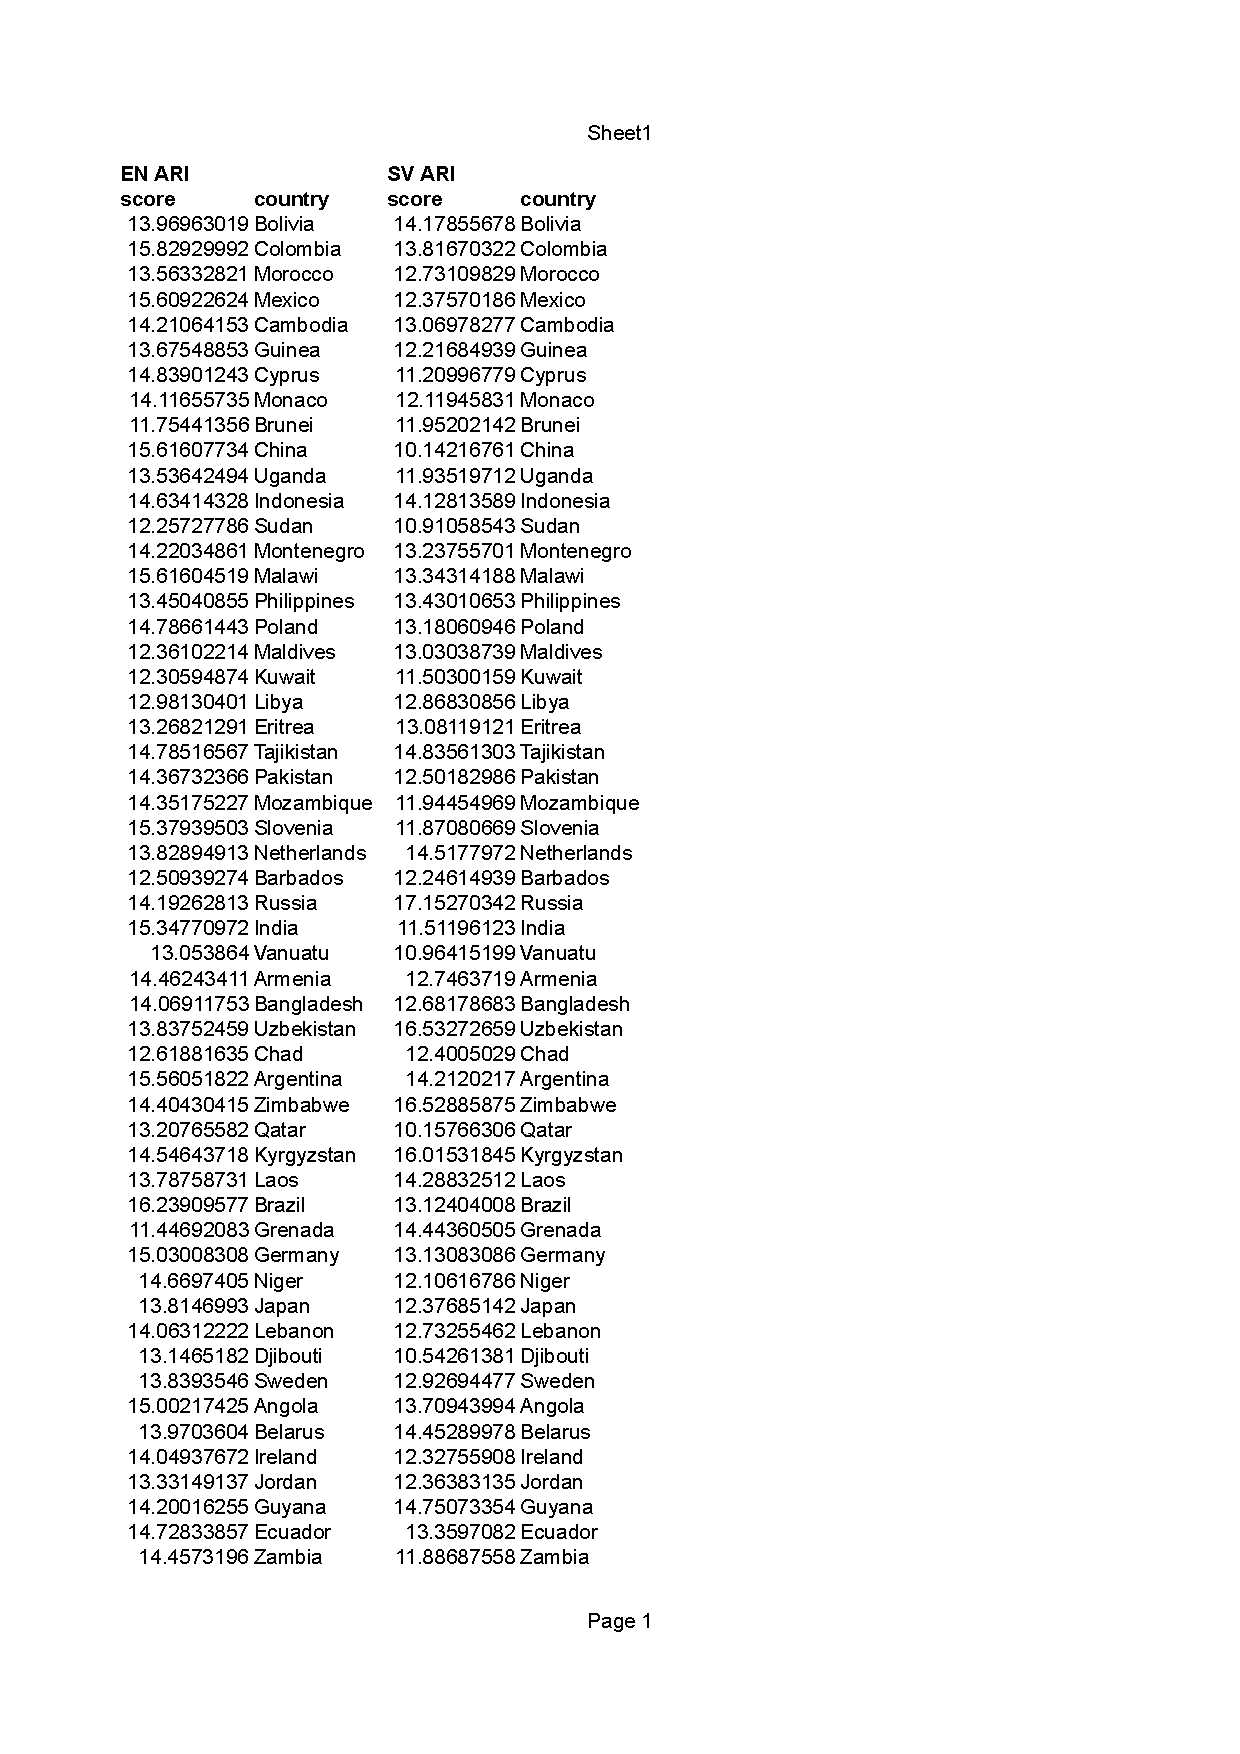
\includegraphics[page=1,scale=0.75]{./DATA/ARI.pdf}
\includegraphics[page=2,scale=0.75]{./DATA/ARI.pdf}
\includegraphics[page=3,scale=0.75]{./DATA/ARI.pdf}

\newpage
\subsection{CLI}
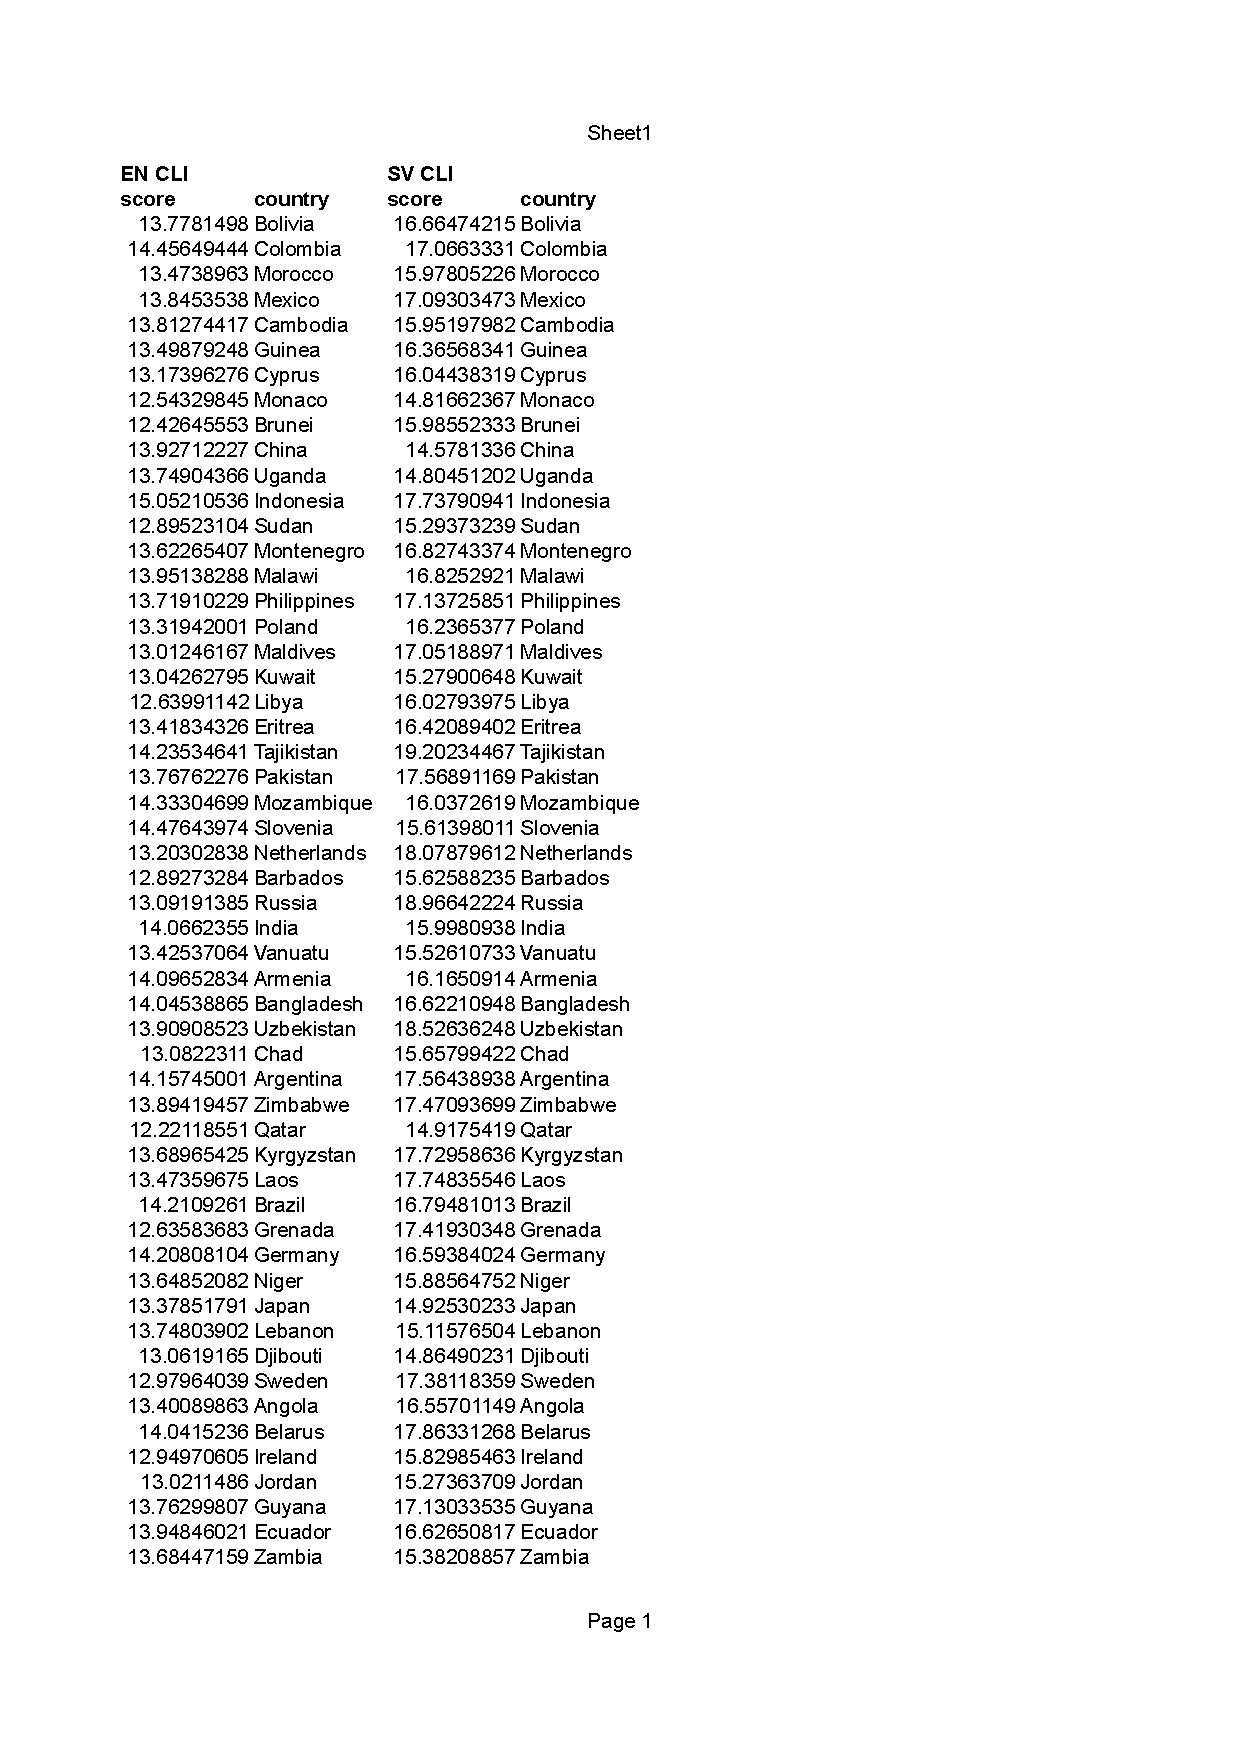
\includegraphics[page=1,scale=0.75]{./DATA/CLI.pdf}
\includegraphics[page=2,scale=0.75]{./DATA/CLI.pdf}
\includegraphics[page=3,scale=0.75]{./DATA/CLI.pdf}

\newpage
\subsection{LIX}
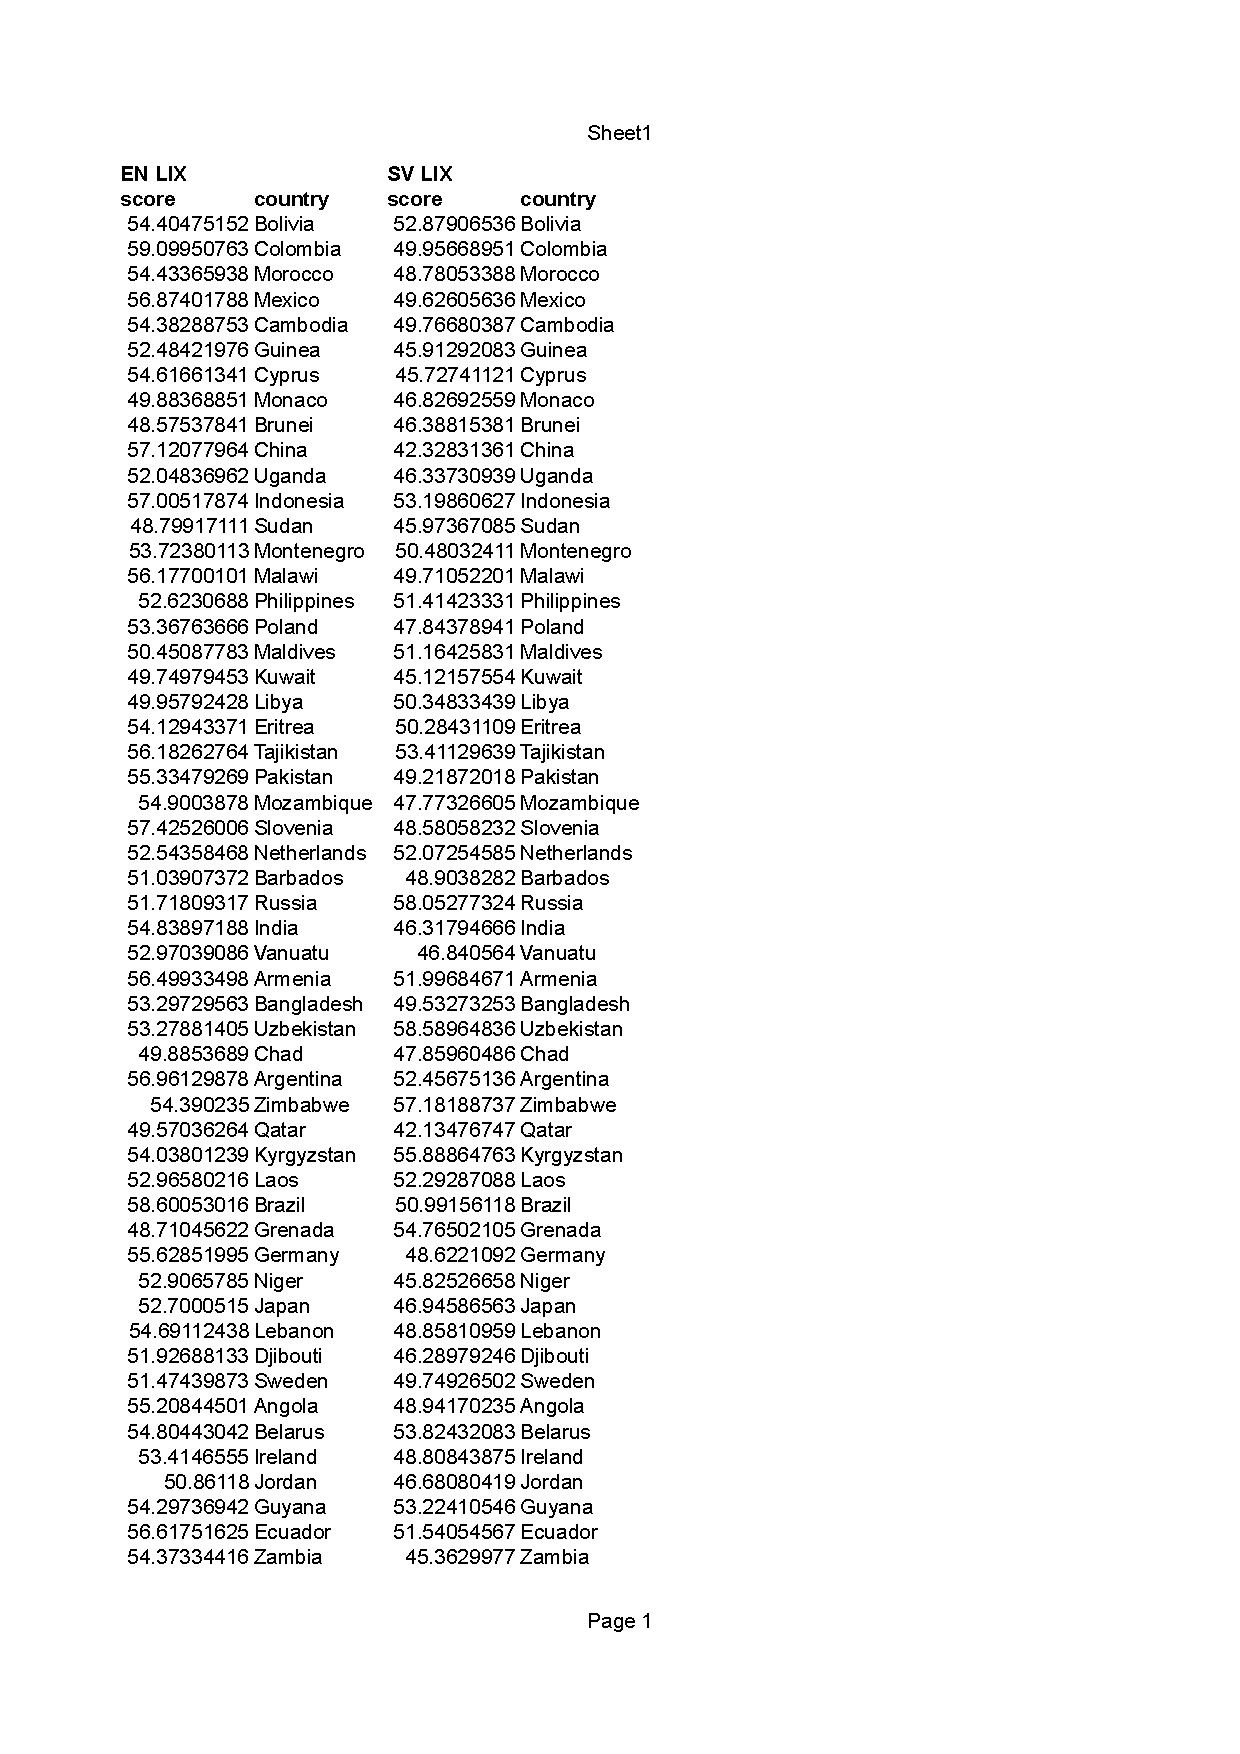
\includegraphics[page=1,scale=0.75]{./DATA/LIX.pdf}
\includegraphics[page=2,scale=0.75]{./DATA/LIX.pdf}
\includegraphics[page=3,scale=0.75]{./DATA/LIX.pdf}

\end{document}